\documentclass{beamer}%Do not change this
\usepackage{hyperref}%Enables hyperlinks
\usepackage{graphicx}%To add images
\usepackage{animate}
\setbeamertemplate{footline}[frame number] %Adds frame numbers to footnote area
\setbeamertemplate{bibliography item}[text] %Makes the bibliography display properly
%Leave the lines above

\hypersetup{
  colorlinks=true,
  linkcolor=green,
  urlcolor=green
}

\usetheme{Rochester}
\usecolortheme{seagull}
\setbeamersize{text margin left=8mm,text margin right=8mm}
\definecolor{cyberpunkyellow}{HTML}{FCEE09}
\definecolor{cyberpunkdark}{HTML}{101820}
\setbeamercolor{title}{fg=cyberpunkdark,bg=cyberpunkyellow}
\setbeamercolor{frametitle}{fg=cyberpunkdark,bg=cyberpunkyellow}

\title{Ethics of Connected Technology}
\subtitle{Who Bears the Risks When Technology Fails?}
\author{Quinton Baudoin \\ Caylei Dauphiney \\ Royce Diano \\ Connor Segura}
\date{Fall 2026} %Leave this as-is

\begin{document}
\begin{frame}[plain,t]
\centering
\makebox[\linewidth]{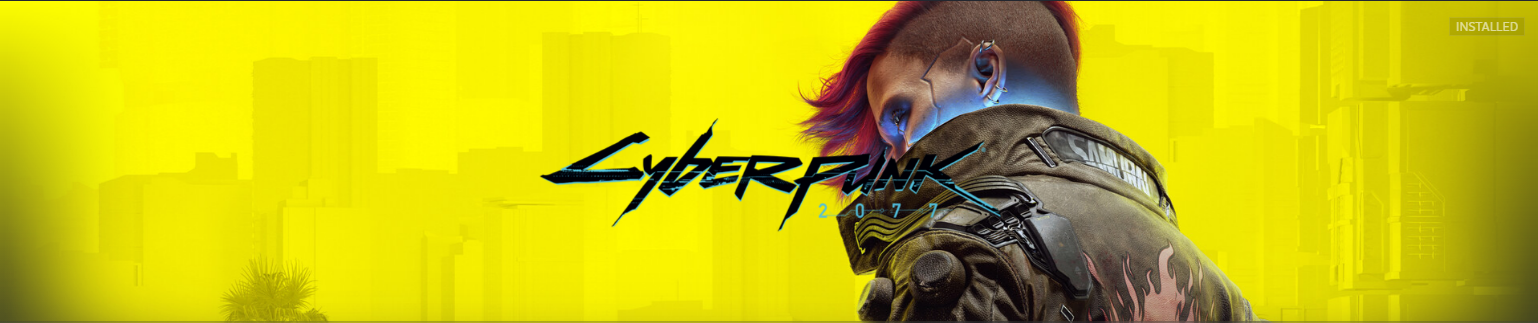
\includegraphics[width=\paperwidth]{presentation-cover.png}}
\titlepage
\end{frame}

\begin{frame}
\frametitle{The Ethical Stakes}
\begin{itemize}
  \item Networked AI, cyberware, and hacking promise powerful benefits.
  \item In Night City, security failures expose people to risks they did not choose.
  \item The people most exposed often have the least power, protection, or recourse.
\end{itemize}
\bigskip
\centering
\textbf{Security, oversight, and equitable access are design requirements--not optional extras.}
\end{frame}

\begin{frame}
\frametitle{The Datakrash: Failure at Network Scale}
\begin{itemize}
  \item R.A.B.I.D.S. breached corporate data fortresses, triggering cascading failures across the global Net.
  \item Rogue AIs escaped into a damaged network; communications and digital services broke down.
  \item Secrecy and a single containment barrier could not protect the public from systemic failure.
\end{itemize}
\bigskip
\textbf{Ethical response:} independently test containment, isolate critical services, restrict dangerous capabilities, and rehearse recovery before deployment.
\end{frame}

\begin{frame}
\frametitle{The Blackwall Isn't Perfect}
\begin{itemize}
  \item The Blackwall limits exposure to rogue AIs, but does not guarantee complete isolation.
  \item The Voodoo Boys expose V to danger beyond the Blackwall without informed consent.
  \item Public protection must include oversight of security powers and a voice for affected communities.
\end{itemize}
\bigskip
\textbf{Before high-risk access:} require independent approval, documented precautions, and plans to notify and assist affected people.
\end{frame}

\begin{frame}
\frametitle{Cyberware: Health, Access, and Control}
\begin{columns}[T]
\column{0.56\linewidth}
\begin{itemize}
  \item Cyberware can restore bodily function--but safe repairs and upgrades depend on wealth.
  \item Vendor-controlled updates, repairs, or disconnection can threaten bodily autonomy.
  \item A quickhack against an implant can turn a software flaw into physical injury.
\end{itemize}
\column{0.40\linewidth}
\centering
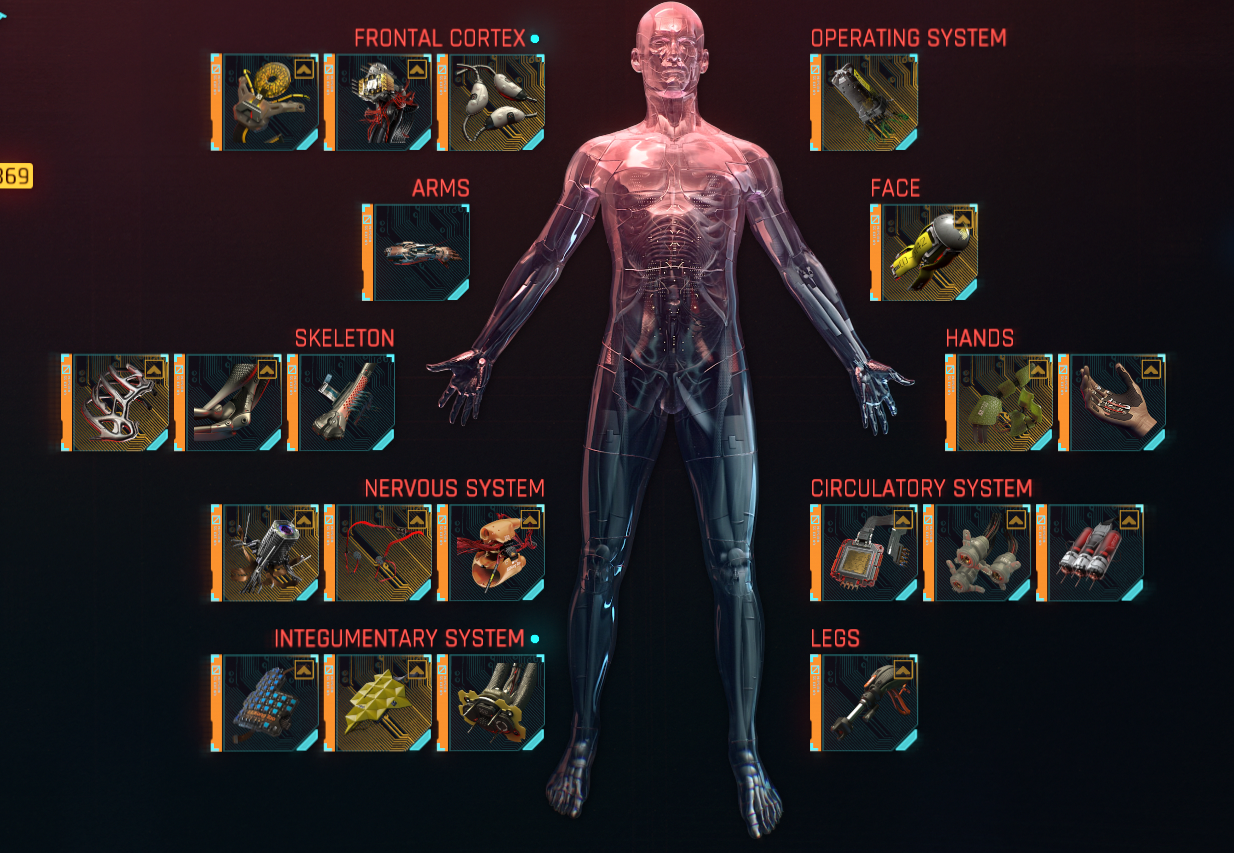
\includegraphics[width=\linewidth]{presentation-cyberware.png}
\end{columns}
\end{frame}

\begin{frame}
\frametitle{Cyberpsychosis: Prevention Before Force}
\begin{columns}[T]
\column{0.56\linewidth}
\begin{itemize}
  \item MaxTac's lethal response treats a crisis as a threat to eliminate.
  \item Regina seeks less lethal outcomes, but individual intervention is not a public health system.
  \item Prioritize prevention, accessible mental-health care, and accountability for knowingly installing faulty cyberware.
\end{itemize}
\column{0.40\linewidth}
\centering
\newlength{\spritewidth}
\newlength{\spriteheight}
\settowidth{\spritewidth}{
\includegraphics{IMAGES/Cyberpsychosis-frames.png}}
\settoheight{\spriteheight}{
\includegraphics{IMAGES/Cyberpsychosis-frames.png}}
\begin{animateinline}[autoplay,loop,poster=first]{10}
\multiframe{24}{iFrame=0+1}{%
  \pgfmathtruncatemacro{\framecol}{mod(\iFrame,4)}%
  \pgfmathtruncatemacro{\framerow}{floor(\iFrame/4)}%
  \pgfmathtruncatemacro{\framecolremaining}{3-\framecol}%
  \pgfmathtruncatemacro{\framerowremaining}{5-\framerow}%
  \edef\frameimage{\noexpand
\includegraphics[width=\the\linewidth,clip,trim={%
    \the\dimexpr\spritewidth*\framecol/4\relax\space
    \the\dimexpr\spriteheight*\framerowremaining/6\relax\space
    \the\dimexpr\spritewidth*\framecolremaining/4\relax\space
    \the\dimexpr\spriteheight*\framerow/6\relax}]{IMAGES/Cyberpsychosis-frames.png}}%
  \frameimage%
}
\end{animateinline}
\end{columns}
\end{frame}

\begin{frame}
\frametitle{Connected Devices Need Lifecycle Security}
\begin{itemize}
  \item The FDA recommends cybersecurity risk management, effective-control testing, and clear end-of-support information for medical devices \cite{FDA2026}.
  \item NIST's IoT baseline identifies data protection, restricted logical access, and secure software updates as core capabilities \cite{NIST2020}.
  \item The report recommends making these capabilities baseline expectations for connected medical devices.
\end{itemize}
\bigskip
\textbf{Fairness matters too:} guarantee repair and support for medically necessary devices; do not make safe operation depend on a user's ability to pay.
\end{frame}

\begin{frame}
\frametitle{Hacking Threatens Privacy and Essential Services}
\begin{itemize}
  \item Ping turns nearby devices into surveillance opportunities--even for people who never chose to connect.
  \item Netrunner attacks show how digital compromise can cause physical harm or interrupt services.
  \item NIST recommends protecting device interfaces and data from unauthorized access and modification \cite{NIST2020}.
\end{itemize}
\bigskip
\textbf{Beyond technical controls:} minimize data collection, give meaningful notice and control, separate critical systems, and rehearse safe recovery.
\end{frame}

\begin{frame}
\frametitle{Netrunners: Cyberdecks and Quickhacks}
\begin{columns}[T,onlytextwidth]
\column{0.30\textwidth}
\centering

\includegraphics[width=\linewidth,height=0.56\textheight,keepaspectratio]{IMAGES/Cyberdeck.png}

\small Cyberdeck: enables quickhacks
\column{0.30\textwidth}
\centering

\includegraphics[width=\linewidth,height=0.56\textheight,keepaspectratio]{IMAGES/PING.png}

\small Ping: reveals connected targets
\column{0.30\textwidth}
\centering

\includegraphics[width=\linewidth,height=0.56\textheight,keepaspectratio]{IMAGES/Cyberware Malfunction.png}

\small Cyberware Malfunction: disables implants
\end{columns}
\end{frame}

\begin{frame}
\frametitle{What Responsible Technology Requires}
\begin{enumerate}
  \item \textbf{Prevent:} secure defaults, independent testing, and least-privilege access.
  \item \textbf{Protect:} isolate critical services and safeguard users throughout a device's life.
  \item \textbf{Share fairly:} provide accessible care, maintenance, and repair.
  \item \textbf{Answer for harm:} document decisions, notify affected people, and provide oversight and recourse.
\end{enumerate}
\end{frame}

\begin{frame}
\frametitle{Conclusion}
\begin{itemize}
  \item The technologies are fictional; the obligations are not.
  \item People should not carry risks created by systems they cannot inspect, control, or afford to protect.
  \item Ethical deployment means safe failure, durable support, equitable access, and accountability to affected communities.
\end{itemize}
\end{frame}

\begin{frame}
\frametitle{Sources}
\bibliography{citations}
\bibliographystyle{ieeetr}
\end{frame}

\end{document}
